\documentclass{whutmod}
\usepackage[linesnumbered,ruled,lined]{algorithm2e}
\bibliographystyle{unsrt}
\team{10}
\membera{刘子川}
\joba{编程}
\memberb{程宇}
\jobb{建模}
\memberc{祁成}
\jobc{写作}
\hypersetup{
	colorlinks=true,
	linkcolor=black,citecolor=black
}

\newcommand{\udots}{\mathinner{\mskip1mu\raise1pt\vbox{\kern7pt\hbox{.}}  
		\mskip2mu\raise4pt\hbox{.}\mskip2mu\raise7pt\hbox{.}\mskip1mu}} 

\newcommand{\upcite}[1]{\textsuperscript{\cite{#1}}}
%%%%%%%%%%%%%%%%%%%%%%%%%%%%%%%%%题目%%%%%%%%%%%%%%%%%%%%%%%%%%%%%%%%%%%%
\title{基于xxxxxxxx模型}
\tihao{1} 

\begin{document}

	\maketitle
	\thispagestyle{empty}
%%%%%%%%%%%%%%%%%%%%%%%%%%%%%%%%%摘要%%%%%%%%%%%%%%%%%%%%%%%%%%%%%%%%%%%%
	\begin{abstract}
		控制高压油管的压力变化对减小燃油量偏差,提高发动机工作效率具有重要意义。本文建立了基于质量守恒定理的微分方程稳压模型,采用二分法、试探法以及自适应权重的蝙蝠算法对模型进行求解。
		//
	
		针对问题一,建立基于质量守恒定律的燃油流动模型,考察单向阀开启时间对压力稳定性的影响。综合考虑压力与弹性模量、密度之间的关系,提出燃油压力-密度微分方程模型和燃油流动方程。本文采用改进的欧拉方法对燃油压力-密度微分方程求得数值解;利用二分法求解压力分布。综合考虑平均绝对偏差等反映压力稳定程度的统计量,求得直接稳定于100MPa的开启时长为\textbf{0.2955ms} ,在2s、5s内到达并稳定于150MPa时开启时长为\textbf{0.7795ms}、\textbf{0.6734ms},10s到达并稳定于150MPa的开启时长存在多解。最后对求解结果进行灵敏度分析、误差分析。
		//
	
		针对问题二,建立基于质量守恒定律的泵-管-嘴系统动态稳压模型,将燃油进入和喷出的过程动态化处理。考虑柱塞和针阀升程的动态变动,建立喷油嘴流量方程和质量守恒方程。为提高角速度求解精度,以凸轮转动角度为固定步长,转动时间变动步长,采用试探法粗略搜索与二分法精细搜索的方法求解,求得凸轮最优转动角速度\textbf{0.0283rad/ms(转速270.382转/分钟)},并得到该角速度下高压油管的密度、压力周期性变化图。对求解结果进行误差分析与灵敏度分析,考察柱塞腔残余容积变动对高压油管压力稳态的影响。
		//
	
		针对问题三,对于增加一个喷油嘴的情况,改变质量守恒方程并沿用问题二的模型调整供、喷油策略,得到最优凸轮转动角速度为\textbf{0.0522rad/ms(498.726转/分钟)};对于既增加喷油嘴又增加减压阀的情况,建立基于自适应权重的蝙蝠算法的多变量优化模型,以凸轮转动角速度、减压阀开启时长和关闭时长为参数,平均绝对偏差MAD为目标,在泵-管-嘴系统动态稳压模型的基础上进行求解,得到最优参数:\textbf{角速度0.0648 rad/ms(619.109转/分钟)}、减压阀的开启时长\textbf{2.4ms}和减压阀的关闭时长\textbf{97.6ms}。
		//
	
		本文的优点为:1. 采用试探法粗略搜索与二分法精细搜索结合的方法,降低了问题的求解难度。2.以凸轮转动角度为固定步长,对不同角速度按照不同精度的时间步长求解,大大提高了求解的精确度。 3.针对智能算法求解精度方面,采用改进的蝙蝠算法,使速度权重系数自适应调整,兼顾局部搜索与全局搜索能力。
		
		\keywords{
			微分方程\quad
			微分方程\quad	
			微分方程\quad
			微分方程\quad
		}
	\end{abstract}


%%%%%%%%%%%%%%%%%%%%%%%%%%%%%%%%%目录%%%%%%%%%%%%%%%%%%%%%%%%%%%%%%%%%%%%
	\thispagestyle{empty}
	\tableofcontents
	\setcounter{page}{0}                                               
	\newpage	%换页符
	

	
	\section{问题重述}	
		\subsection{问题背景}
%	    	分析研究\upcite{1}。xxxxxxxxxxx\footnote{\quad xxxxxxxxxx.}.
	
自动指纹识别系统(automated fingerprint identification system,简称 AFIS)有着广泛的应用背景。目前对自动 指纹识别系统的研究主要有 3 个方面,即图像增强、指纹分类和细节匹配。一般可以分成"离线部分"和"在线部分"两个部分。如图 \ref{lssct} 所示,离线部分包括用指纹采集仪采集指纹、提取出细节点、将细节点保存到数据库中形成指纹模板库等主要步骤。在线部分包括用指纹采集仪采集指纹、提取出细节点、然后将这些细节点与保存在数据库中模板细节点进行匹配,判断输入细节点与模板细节点是否来自同一个手指的指纹\upcite{1,3}。指纹分类一般是用在大规模的指纹库中,作为细节匹配中减少搜索范围的步骤使用。指纹图像一般占用较多的空间,且图像中的像素信息并不适合计算机进行分析或匹配。为实现计算机自动识别,需要有一种方法来描述指纹的内在结构、具体形态和其它特征并将其用最少的字节数来存储于计算机中。此计算机系统可扫描犯罪现场采集的指纹,并且与州、地区、国家之间执法机关采集的数百万指纹档案互相比对\upcite{2}。指纹由专家追踪后,经计算机扫描,得到许多细节来和数据库里其它指纹比对,列出相符合的百分比来让鉴识人员得知可能的相符人选\footnote{\quad https://baike.baidu.com/item/AFIS/2851410?fr=aladdin}。任何计算机比对的结果,都会经指纹专家比较与此指纹相关的样本来验证。
\begin{figure}[H]
	\centering
	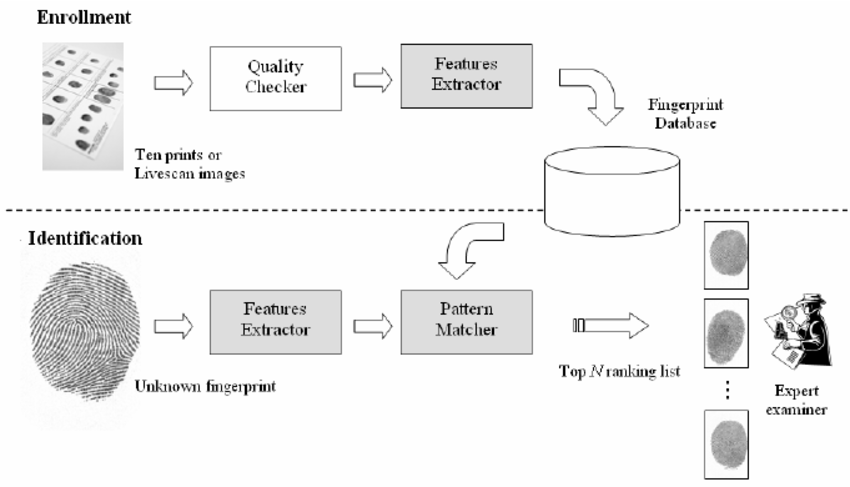
\includegraphics[width=.8\textwidth]{figures/AFIS.png}
	\caption{自动指纹识别系统框图 }\label{lssct}
\end{figure}

		\subsection{问题概述}
		    围绕相关附件和条件要求,试根据附件中的16幅指纹图像,不借助现有的指纹相关软件,依次提出以下问题:
				 
			\textbf{编码:} 给出一种用不超过200字节(下面称为“指纹密码”)来刻画描述指纹基本特征的表示方法,介绍其数学原理。
			
			\textbf{匹配:} 将你的方法编程实现,对附件中的每一幅指纹都给出其“指纹密码”的表示。基于你找到的这些指纹表示,你能否给出一种方法比较不同指纹间的异同及相似程度?
			
			\textbf{应用:} 你能否对附件中的16个指纹进行对比和归类?请给出你对比及分类的依据和结果。

	\section{模型假设}
		\begin{itemize}                                             
		\item [(1)] 
		\item [(2)]
		\item [(3)] 
		\item [(4)] 
		\end{itemize}

		
	\section{符号说明}
		\begin{table}[H]
		\centering
		\setlength{\tabcolsep}{12mm}
		\begin{tabular}{cc}
			\toprule[1.5pt]
			\multicolumn{1}{m{5cm}}{\centering 符号} & \multicolumn{1}{m{5cm}}{\centering 说明} \\
			\midrule[1pt]		
			$P_n$  & 20个站点  \\ 
			$P_n$  & 20个站点  \\ 
		   	$P_n$  & 20个站点  \\ 
			\bottomrule[1.5pt]
		\end{tabular}
		\begin{tablenotes}
		\item 注:表中未说明的符号以首次出现处为准
		\end{tablenotes}
		\end{table}

	\section{问题一模型的建立与求解}
		\subsection{数据预处理}
		在正式搭建模型前,本文首先将图片进行预处理,以方便进行后续运算。经过归一化处理,???和???后,即可得到相同规格的二值化图片。
		\subsubsection{归一化处理}
		\paragraph{灰度值处理}
		鉴于各个指纹图像的纹理深浅不统一,首先对每张图片做灰度值归一化处理。对于图片$P_{i}$,其第$x$行第$y$列的像素点的灰度值可表示为$P_{i}(x,y)\in[0,255]$。即当$P_{i}(x,y)=255$时,$P_{i}(x,y)$为纯白色像素点;当$P_{i}(x,y)=0$时,$P_{i}(x,y)$为纯黑色像素点。对于任意图片$P_{i}$,有
		\begin{gather*}
		P_{i,max}=\underset{1\leqslant x\leqslant n,1\leqslant y \leqslant  m}{max}P_{i}(x,y),\\
		P_{i,min}=\underset{1\leqslant x\leqslant n,1\leqslant y \leqslant  m}{min}P_{i}(x,y),
		\end{gather*}
		其中$n$和$m$分别表示图片的行数和列数。即	$P_{i,max}$与$P_{i,min}$分别表示图片中像素的最大灰度值和最小灰度值。对图片执行线性归一化操作如下
		\begin{gather*}
     	P_i(x,y)'=\frac{255}{P_{i,max}-P_{i,min}}(P_i(x,y)-P_{i,min})
		\end{gather*}
		即将图片$P_i$像素点灰度值线性放缩于$[0,255]$间,得到灰度值归一化图片$P_i'$。
	    
	  	\paragraph{外框去除与尺度统一}
	  	对于图片$P_{i}$,我们将去除其空白外框以方便后续学习策略运算。设定边界阈值为$threshold_N$,当图片$P_{i}$最上方的某一行和最下方的某一行的非空白像素数大于$threshold_N$时,将其定义为新的上边界或下边界,及可得到行边界位置如下
	    \begin{gather*}
	  	fringe_{x1}=\underset{ (\sum_{i=1}^{m} (P'(x,i)<255))>threshold_N}{max(x)},\\
	  	fringe_{x2}=\underset{(\sum_{i=1}^{m} (P'(x,i)<255))>threshold_N}{min(x)}
	  	\end{gather*}
	  	其中$fringe_{x1}$与$fringe_{x2}$ 分别为新定义上边界与下边界,同理有列边界位置如下
	   \begin{gather*}
	  	fringe_{y1}=\underset{(\sum_{i=1}^{n} (P'(i,y)<255))>threshold_N}{min(y)},\\
	  	fringe_{y2}=\underset{(\sum_{i=1}^{n} (P'(i,y)<255))>threshold_N}{max(y)}
	  	\end{gather*}
	  	其中$fringe_{y1}$与$fringe_{y2}$分别为新定义左边界与右边界。即去除外框后的图片可表示为	$P''=P'(	fringe_{x1}:	fringe_{x2},	fringe_{y1}:	fringe_{y2})$。即只保留新定义边界内的像素点并删除剩余像素点即可得到去除外框后的图片$P''_{i}$。定义标准行数为$N$,标准列数为$M$,将去除外框后的图片$P''_{i}$进行放缩处理可得归一化图片$P_{i}^s$如下
	  	\begin{gather*}
	  	P_{i}^s(x,y)=P''_{i}(floor(\frac{fringe_{x1}-fringe_{x2}}{N}x),floor(\frac{fringe_{y2}-fringe_{y1}}{M}y))\\
	  	x\in[1,N],	y\in[1,M]
	  	\end{gather*}
	  	其中$floor$表示向下取整,即通过灰度值处理、外框去除与尺度统一后即可将原始指纹图片数据$P_{i}$转换为灰度值范围与图片尺度统一的归一化图片数据$P_{i}^s(x,y)$。
	  	\subsubsection{图像强化处理}
	  	利用Grunward-Letnikov微分算子,构造自适应函数,采集梯度信息和计算信息熵,从而确定微分阶数。	
	  	为了确定自适应分数阶微分阶数$v$,需要确定每个像素的梯度$G$和信息熵$E$。
	  	梯度$G$反映指纹像素特征在感兴趣区域(ROI, Region of Interest)上的突变情况,取近似梯度模值为
	  	\begin{gather}
	  	\displaystyle G[f(x,y)]=\max\begin{Bmatrix}
	  	|\frac{\partial f }{\partial x}|,|\frac{\partial f}{\partial y}|
	  	\end{Bmatrix}
	  	\end{gather}
	  	另一个描述图像边缘纹理变化的指标是信息熵$E$,即所有可能发生事件的信息量期望之和,其数学描述为
	  	\begin{gather}
	  	E=-\sum_{i=1}^{n}p(x_i)\cdot log_2(p(x_i))	
	  	\end{gather}
	  	其中,$p(x_i)$是事件$x_i$发生的概率,$n$是可能发生事件的个数。对信息熵进行归一化处理,可以获得取值范围为$[0,1]$的信息熵
	  	\begin{gather}
	  	\displaystyle E'=\frac{E-E_{min}}{E_{max}-E_{min}}
	  	\end{gather}
	  	综合梯度模值和信息熵,构造关系函数$v=w_1\cdot G+w_2\cdot E'+w_3$,即微分阶数$v$由梯度和信息熵共同决定,梯度模值和信息熵越大,反映该指纹像素需要增强的程度越大,更可能为纹理区域或边缘,分数阶微分阶数取值也越大。此问题中,
	  	
	  	\begin{gather}
	  	\displaystyle\frac{\partial^v f(x,y)}{\partial x_{i}^{v}}\doteq\displaystyle\sum_{k=0}^{x_i-v}(-1)^{k}\begin{pmatrix}
	  	l \\ k
	  	\end{pmatrix}f(x_i-k) 
	  	\end{gather}
	  	$x_i(i=0,1,...,7)$是不同的偏微分方向,此处取以$x$轴正向为起始方向,顺时针旋转一周均匀分部的8个方向。为方便计算,此处$x_i-v$取$3$。分别在$8$个方向采用分数阶微分近似掩膜,从而提高图像质量。
	  
	  	
	  	\subsubsection{滤波}
	    \subsubsection{二值化处理}	  	
	    \paragraph{场方向估计}
	    一般指纹图像都有较为清晰的场方向,对于图像上的每一个像素$P(x,y)$,为了确定其在该像素处脊线的方向,以该像素为中心的$9\times9$像素矩阵$u_{P(x,y)}$内,分别计算$8$个
	    方向上的灰度平均值,即对于
	    \begin{gather*}
	  u_{P(x,y)}=\begin{bmatrix}
	  P(x-4,y-4) & \cdots  & P(x,y-4) & \cdots  & P(x+4,y-4) \\ 
	  \vdots & \udots & \vdots  &  \ddots  & \vdots\\ 
	   P(x-4,y) & \cdots & P(x,y) &\cdots& P(x+4,y)  \\ 
	   \vdots & \ddots  & \vdots  &  \udots & \vdots\\ 
	  P(x+4,y+4) & \cdots & P(x,y+4) &\cdots& P(x+4,y+4)  
	  \end{bmatrix}
	    \end{gather*}
	    若$u_{P(x,y)}$中存在若干像素点超出原图像边界时,记超出边界的像素点为$P_o$并使得$\left \{ P_o \right \}=255$。并依照图???中的方向,分别计算$8$个方向上的灰度平均值得到$Gmean[i]$,然后将这 $8$ 个平均值按两两垂直的方向分成 $4$ 组,$0 $和 $4$ 一组、$1$ 和 $5$ 一组、$2$ 和 $6$ 一组、$3$ 和 $7$ 一组,计算
	    每组中两个平均值的差值。
	     \begin{gather*}
	  Gdiff[j]=\left | Gmean[j]-Gmean[j+4] \right |,j=1,2,3,4,
	    \end{gather*}
	    差值绝对值相差最大的方向即为脊线方向与其法向,即
	     \begin{gather*}
	  iDir=\left\{\begin{matrix}arg(\underset{i}{max}(Gdiff[j])),\left | P(x,y)-\underset{i}{max}(Gdiff[j]) \right|<\left | P(x,y)-\underset{i}{max}(Gdiff[j+4]) \right|
	  \\ arg(\underset{i}{max}(Gdiff[j]))+4,otherwise
	  \end{matrix}\right.
	    \end{gather*}
	 	\begin{figure}[H]
	 	\centering
	 	
\includegraphics[width=\textwidth]{figures/whut.jpg}
	 	\caption{问题一思维流程图}\label{lct}
	 \end{figure}   
    \paragraph{二值化}
    得到图像每个像素处的方向场后,再依据方向场来对图像进行二值化。若像素$P(x,y)$处的脊线方向为$iDir$,先用估计方向场的方法计算该像素处在方向$iDir$和其法线$iVar=iDir+4$的灰度平均值$ Gmean[iDir]$和$ Gmean[iVar]$,基于此将该像素二值化为
      \begin{gather*}
    P(x,y)=\left\{\begin{matrix}255, Gmean[iDir]\geqslant Gmean[iVar]
    	\\ 0,otherwise
    \end{matrix}\right.
      \end{gather*}
      其中255为二值图像中图像背景和谷线的灰度值,0 为二值图像中图像脊线的灰度值。
		\subsection{问题描述与分析}
			问题一要求
		
			其思维流程图如图~\ref{lct}~所示:
			\begin{figure}[H]
				\centering
				
\includegraphics[width=\textwidth]{figures/whut.jpg}
				\caption{问题一思维流程图}\label{lct}
			\end{figure}
			
		\subsection{模型的建立}
			\begin{gather*}
			d(p_i,p_j)=\left | x_i-x_j \right |+\left | y_i-y_j \right | ,
			\end{gather*}
	
		
		
		\subsection{模型的求解}
			\begin{algorithm}[H]
			 	\caption{Procedure of Apriori}  
			 	\LinesNumbered  
			 	\setstretch{0.9}   %设置表的行间距
			 	\KwIn{item data base: $D$\newline
			 		minimum Support threshold: $Sup_{min}$\newline
			 		minimum Confidence threshold: $Conf_{min}$
			 	}
			 	\KwOut{frequent item sets $F$}  
			 	\textbf{Initialize} \newline
			 	iteration $t\leftarrow 1$ \newline
			 	The candidate FIS:$C_{t}=\varnothing$ \newline
			 	The length of FIS:$length=1$ \newline
			 	\For{i=1 to sizeof(D)}
			 	{$I_{i}$=D(i)\newline
			 		n=sizeof($I_{i}$)\newline
			 		\For{j=1 to n}{
			 			\If{$I_{i}(j)\notin C_{t}$ }
			 			{$C_{t}=C_{t}\cup I_{i}(j) $}
			 		}
			 	}
			 	$F_{t}=\left \{ f|f\in C_{t},Sup(f)>Sup_{min}\right \}$\newline
			 	\While{$F\neq \varnothing$}
			 	{ t=t+1\newline 
			 		length=length+1\newline	
			 		$C_{t}\leftarrow $ all candidate of FIS in $F_{t-1}$\newline
			 		$F_{t}=\left \{ f|f\in C_{t},(Sup(f)>Sup_{min})\bigcap (Comf(f)>Conf_{min}) \right\}$\newline
			 	}	
			 	\Return{$F_{t-1}$} 
			\end{algorithm} 
		
        \subsection{实验结果及分析}
  
	\section{问题二模型的建立与求解}
		\subsection{问题描述与分析}
			问题二要求

    		其思维流程图如图~\ref{lssssct}~所示:

			\begin{figure}[H]
				\centering
				
\includegraphics[width=\textwidth]{figures/whut.jpg}
				\caption{问题二思维流程图}\label{lssssct}
			\end{figure}

		\subsection{模型的建立}
		
		\subsection{模型的求解}

        \subsection{实验结果及分析}
        
			结果如下表\ref{zhuanssssasgzai}所示:
			\begin{table}[H]
			\setstretch{1.4}  %设置表的行间距
			\centering		
			\caption{xxxxxxxxxxxxxxxxxxxxx}\label{biao1}
			\begin{tabular}{cc}
			\toprule[2pt]
				\multicolumn{1}{m{5cm}}{\centering xxxxxxx}
				& \multicolumn{1}{m{5cm}}{\centering xxxxxxx}
				\\
				\midrule[1pt]
				xxxxxxx &   909.80\\ 
				xxxxxxx & 	852.60\\ 
			\bottomrule[2pt]	
			\end{tabular}
			\end{table}
  
  			由表\ref{biao1}可知

			其各个小车的运输细节图下图所示:
			\begin{figure}[H]
				\centering
				\subfigure{
\includegraphics[height=8cm,width=7.5cm]{figures/whut.jpg}}
				\subfigure{
\includegraphics[height=8cm,width=7.5cm]{figures/whut.jpg}}
			\end{figure}	
			\begin{figure}[H]	
				\centering
				\subfigure{
\includegraphics[height=8cm,width=7.5cm]{figures/whut.jpg}}
				\subfigure{
\includegraphics[height=8cm,width=7.5cm]{figures/whut.jpg}}
				\caption{xxxxxxxxxxxxxxxxxxxxxxxxx}
				\label{fisg}
			\end{figure}

    \section{问题三模型的建立与求解}
  		\subsection{结果分析}
  
  	\section{灵敏度分析}
 
  	\section{模型的评价}
		\subsection{模型的优点}
			\begin{itemize}                                             
			\item [(1)]
			\item [(2)] 	
			\end{itemize}
		\subsection{模型的缺点}

  		\subsection{模型改进}

  
  
 
	\newpage	%换页符
	%%参考文献
	%\begin{thebibliography}{9}%宽度9
	% \setlength{\itemsep}{-2mm}
	\nocite{*}		%排版未引用的参考文献
	\begin{thebibliography}{9}%宽度9
		\bibitem{1}Davies S G. Touching Big Brother: How biometric technology will fuse flesh and machine[J]. Information Technology \& People, 2014, 7(4): 38-47.
	\bibitem{2}Moses K R, Higgins P, McCabe M, et al. Automated fingerprint identification system (AFIS)[J]. Scientific Working Group on Friction Ridge Analysis Study and Technology and National institute of Justice (eds.) SWGFAST-The fingerprint sourcebook, 2011: 1-33.
	\bibitem{3}Dror I E, Wertheim K, Fraser‐Mackenzie P, et al. The impact of human–technology cooperation and distributed cognition in forensic science: biasing effects of AFIS contextual information on human experts[J]. Journal of forensic sciences, 2012, 57(2): 343-352.
	\bibitem{4}
	\bibitem{5}
	\end{thebibliography}

	\newpage
	%附录
	\appendix %%附录
	\section{数据可视化的实现}
		\subsection*{第一问画图--python源代码}
			\begin{lstlisting}[language=python]
			
			\end{lstlisting}
			
		\subsection*{第二问画图--python源代码}
			\lstinputlisting[language={python},numbers=left,numberstyle=\tiny,
			rulesepcolor=\color{red!20!green!20!blue!20},  
			keywordstyle=\color{blue!70!black},  
			commentstyle=\color{blue!90!},  
			basicstyle=\ttfamily] {./code/demo.py}

\end{document}